\clearpage
\pagenumbering{arabic}
\section{Introduction}\label{introduction}
\gls{perc} is a non-profit organization
authorized by the Propane Education and Research Act of 1996, Public Law 104{-}284.
\gls{perc} was created \textit{“to enhance consumer and employee safety and training, to provide for research and development of clean and efficient propane utilization equipment, and to inform and
	educate the public about safety and other issues associated with the use of propane.”} The Certified Employee Training Program has been the \textit{“gold standard”} of training in the
propane industry for several years. To date, this training has been conducted in a classroom
environment using printed books. After a course, students have the option to sit
for a proctored certification exam, overseen by the National Propane Gas Association.
Now the Certified Employee Training Program is developing an e-learning format of this program to release in 2021.\gls{perc} wants to create and Help Desk, to help their students to face all the possible new challenges.

Switching from the traditional classroom and face-to-face instructor training to computer-based training in a virtual classroom makes the learning experience entirely different for students. Their weak monitors make it hard to follow the course and their learning experience becomes problematic. Moreover, most of them find it difficult to keep in tune with the technical requirements of the chosen course. Also, the lack of computer literacy is a major issue among students today. Many of them cannot operate basic programs such as \textit{\gls{word}}\footnote{From here on, all words in italics will indicate a word in the glossary. You can consult the glossary for more information on that word, concept, or product.} and \textit{\gls{pp}} and therefore are not able to handle their files. Furthermore, many students find fixing basic computer problems troublesome, as they do not know this area. However, technological proficiency is a must for following online courses, as it enables students to manage their assignments and courseware in an organized manner without struggling.

Giglium's leadership thanks to this project will change this state of affairs, socially and technically. On the social front, Giglium will facilitate communication with students and help the troubleshooting process to be quicker thanks to the excellent expert teams brought together by us. On the technical side, Giglium will be the editor and, when necessary, author, of a set of rigorous engineering artifacts fit for refinement into a help desk system. Giglium believes that it will be the social and technical catalyst and glue to keep the project lively, on track, and ensure that it meets the expectations of \gls{perc}.


\begin{figure}[ht!]
	\centering
	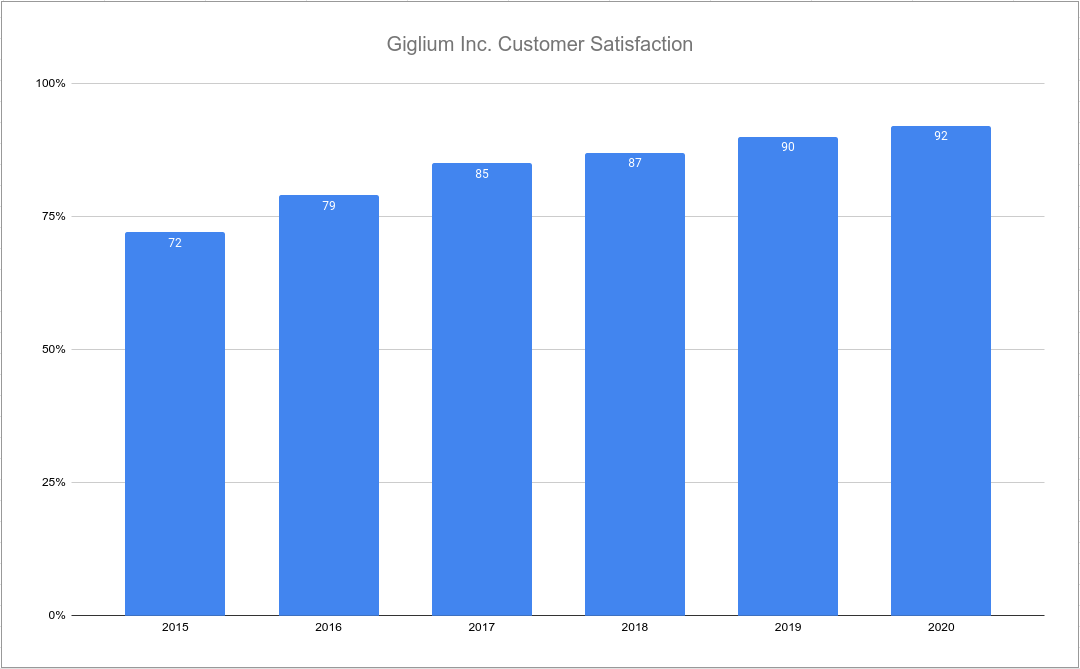
\includegraphics[width=100mm]{./img/introduction/customer-satisfaction-graph.png}
	\caption{Customer Satisfaction: A Giglium Inc.\ Priority}\label{fig:customer-satisfaction}
\end{figure}

\clearpage
The main reasons that Giglium has this belief are multiple. Each year, we hire a third-party research firm to survey hundreds of Giglium customers
worldwide. They are asked what we are doing well and where we need to improve. In Figure~\ref{fig:customer-satisfaction}, as you can see, since we began formally tracking this data, our numbers are strong. In 2020, we reached a possible customer satisfaction score of 92\% out of a possible 100\%, this result was possible since we believe that customers drive our company. And we also believe that we can never be “too close to a customer's needs” or be “listening too much.” It is through our customers that we identify and capture market transitions, measure our success, and design and create solutions. Our customer-centric approach, combined with our culture, is what makes us a “vendor of choice.” Now, at a time when the technology industry is going through a period of dramatic change, Giglum works with the market leader in multiple areas. 
Thanks to this ecosystem of partners, we have earned the trust and satisfaction of our
customers.  

\begin{figure}[ht!]
	\begin{subfigure}{\linewidth}
		
\includegraphics[width=.25\linewidth]{./img/introduction/azure.png}\hfill
		
\includegraphics[width=.25\linewidth]{./img/introduction/gcp.png}\hfill
		
\includegraphics[width=.25\linewidth]{./img/introduction/red-hat.png}
	\end{subfigure}\par\medskip
	\begin{subfigure}{\linewidth}
		
\includegraphics[width=.25\linewidth]{./img/introduction/github.png}\hfill
		
\includegraphics[width=.25\linewidth]{./img/introduction/hashicorp.png}\hfill
		
\includegraphics[width=.25\linewidth]{./img/introduction/jabra.png}
	\end{subfigure}\par\medskip
	\begin{subfigure}{\linewidth}
		
\includegraphics[width=.25\linewidth]{./img/introduction/libraesva.png}\hfill
	\end{subfigure}
	\caption{Giglium, inc.\ partner ecosystem}\label{fig:partner}
\end{figure}

All of these partners are what make Giglium an ideal systems integrator and partner for your digital transformation.
